\section{Wizualizacja systemu i \emph{API}}

\par Aby umożliwić obserwowanie działania systemu powstała \emph{aplikacja webowa}. Jej głównymi zadaniami jest obserwowanie zmian zachodzących w systemie, aby umożliwić wygenerowanie statystyk dotyczących jego działania, jak i pozwolić na wizualizację bieżącego stanu systemu. Interfejs graficzny, został oparty o technologię \emph{React}\cite{REACT_SITE}, z wykorzystaniem paczek \emph{MobX}\cite{MOBX_SITE} oraz \emph{React Leaflet}\cite{REACT_LEAFLET_SITE}.

\par Stworzony w ten sposób interfejs, pozwala na wyświetlanie bieżących pozycji patroli oraz incydentów, które wystąpiły w systemie. Centralna część pozwala na obserwowanie obecnego stanu mapy, natomiast lista po lewej stronie wyświetla działające w systemie patrole wraz z ich stanem. Możliwe jest ich wybranie, aby zostały one zaznaczone na mapie odmiennym kolorem. Nad tą listą znajduje się panel, który wyświetla obecny stan systemu. Wszystkie te elementy możemy zaobserwować na grafice \ref{fig:uiWhole}.

\begin{figure}
    \centering
    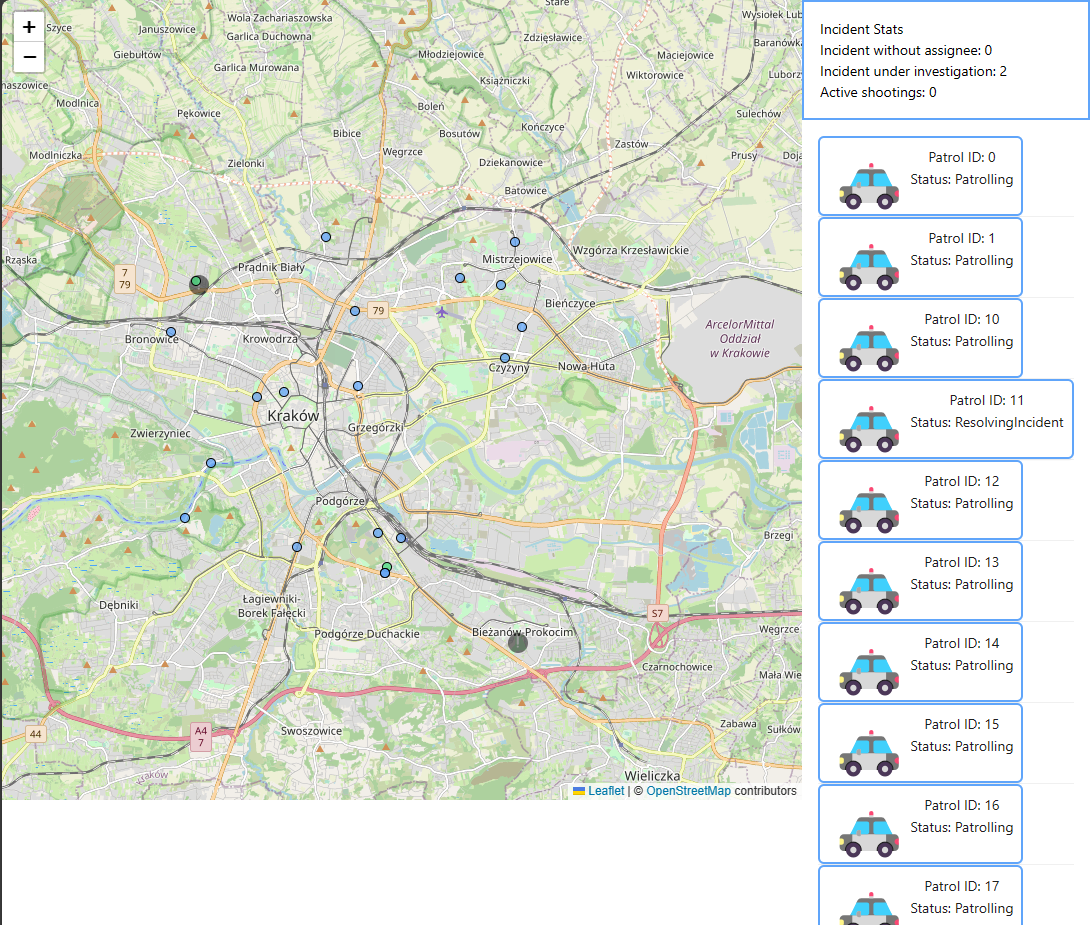
\includegraphics[width=\linewidth]{UI - Whole User Interface}
    \caption{Interfejs użytkownika}
    \label{fig:uiWhole}
    \source{Opracowanie Własne}
\end{figure}

\par Widoczne na mapie znaczniki w kształcie kolorowych kółek, są patrolami. Ich kolor wskazuje na posiadany stan. W systemie wyróżniamy stany:
\begin{itemize}
    \item \emph{Patrolling} - niebieski - oznacza patrol, którego obecnym zadaniem jest patrolowanie wyznaczonego mu obszaru.
    \item \emph{ResolvingIncident} - zielony - oznacza patrol, który został przypisany do konkretnego incydentu.
    \item \emph{InShooting} - czerwony - oznacza patrol, który bierze aktywny udział w strzelaninie lub zmierza, w roli wsparcia, do strzelaniny. W tym stanie prędkość patrolu jest zwiększona i zależy ona od konfiguracji opisanej w podrozdziale \ref{sec:konfiguracja}.
    \item Morski - oznacza patrole, które zostały wybrane, kotrzystając z listy patroli.
\end{itemize}

\par Incydenty zostały oznaczone za pomocą znaczników z wykrzyknikami w środku. Jeżeli wykrzyknik jest czarny, oznacza to, że dane zdarzenie przebiega normalnie. Z kolei, znaczniki posiadające czerwony znak wykrzyknienia, oznaczają strzelaniny.

\begin{figure}
    \centering
    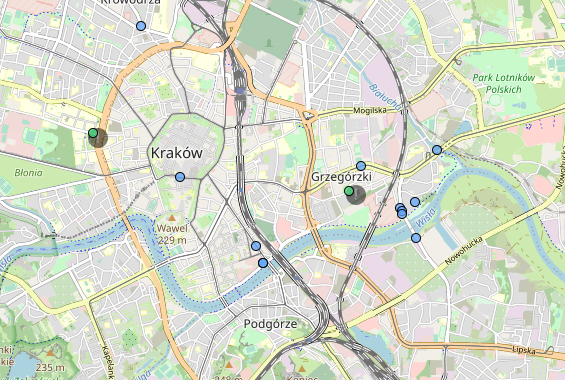
\includegraphics{UI - Patrols - Patrolling and Solving}
    \caption{Patrols - \emph{ResolvingIncident}}
    \label{fig:uiPatrolsPatrollingAndSolving}
    \source{Opracowanie Własne}
\end{figure}

\begin{figure}
    \centering
    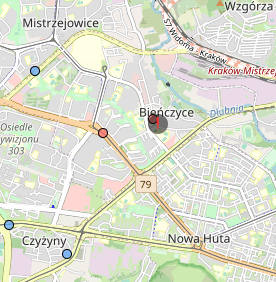
\includegraphics{UI - Patrols - Shooting}
    \caption{Patrols - \emph{InShooting}}
    \label{fig:uiPatrolsInShooting}
    \source{Opracowanie Własne}
\end{figure}

\par Informacje o zmianach, jakie nastąpiły w systemie, wyświetlają się na bieżąco, dzięki zastosowaniu technologii \emph{SignalR}\cite{SIGNALR_SITE}. Dane o nowych incydentach i patrolach, jak i aktualizacje ich stanów i pozycji, są automatycznie wysyłane do podłączonych klientów. Pozwala to na obserwowanie stanu systemu w czasie rzeczywistym.

\par Na podstawie zebranych danych \emph{API} potrafi również wygenerować pliki ze statystykami. Dane zgromadzone w ten sposób, zostały wykorzystane do analizy działania systemu i oceny wpływu informacji kontekstowych na proces decyzyjny. Informacje zawarte w tych plikach to: historia poruszania się patroli, historia stanów patroli, historia przebiegów incydentów, oraz dane wykorzystywane w procesie decyzyjnym, takie jak średnia odległość dostępnych patroli od wybranego incydentu.